\documentclass[tikz]{standalone}
\usepackage[dvipsnames,svgnames,x11names]{xcolor}
\usepackage{tikz}
\usepackage{pgfplots}
\usetikzlibrary{pgfplots.statistics}
\pgfplotsset{compat = 1.12}
\usepackage[
  group-separator={,},
  exponent-product=\cdot,
  binary-units = true,
]{siunitx}
\usepackage{../thesismath}
\begin{document}
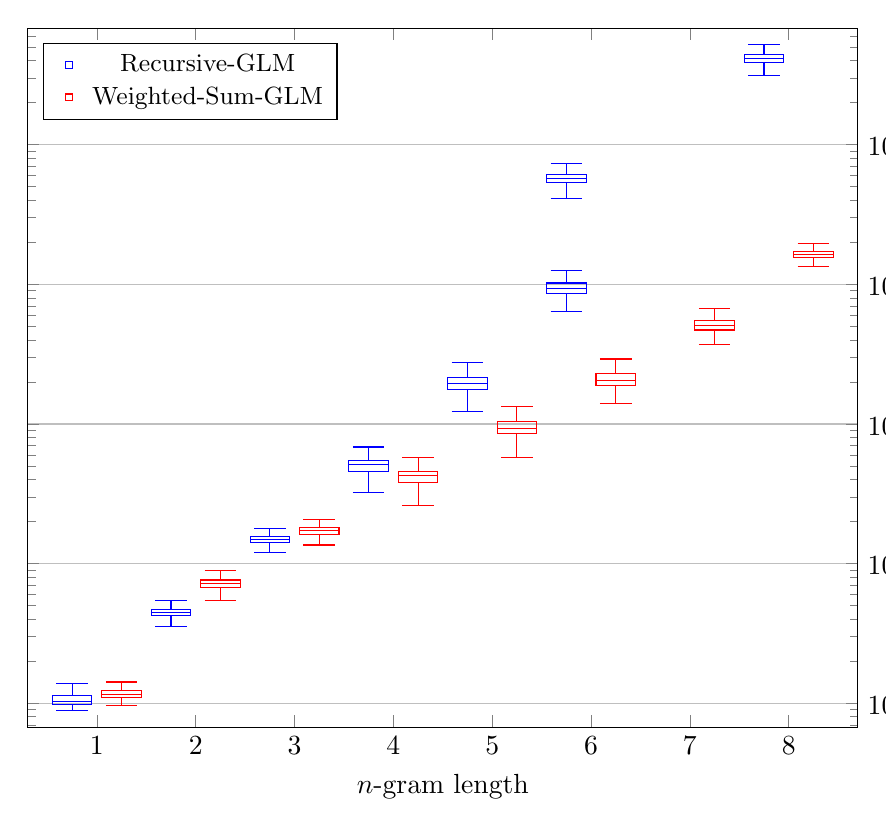
\begin{tikzpicture}[baseline, trim axis left, trim axis right]

\pgfplotscreateplotcyclelist{recglm_glm}{%
  blue,  mark size=1.25, mark=square,\\%
  red,   mark size=1.25, mark=square,\\%
}

\pgfplotsset{
  legend style = {
    legend image code/.code = {
      \draw[only marks]
        plot coordinates {
          (0.3cm,0cm)
        };
      \node at (0.15cm, 0cm) {};
      \node at (0.45cm, 0cm) {};
    },
  },
  boxplot/draw/average/.code = {
    %\draw[dashed, /pgfplots/boxplot/every average/.try]
    %  (boxplot box cs:\pgfplotsboxplotvalue{average},0)
    %  --
    %  (boxplot box cs:\pgfplotsboxplotvalue{average},1)
    %  ;
  },
}

\begin{axis}[
%   title = {Calculation Time per Probability $\ProbGLM{w}{h}$},
  xlabel = {$n$-gram length},
  xtick = {1, ..., 8},
  xmin = 0.5,
  xmax = 8.5,
  ylabel = {Calcluation Time [\si{\micro\second}]},
  yticklabel pos = right,
  ymax = 0.886,
  ymax = 51890.229,
  ymode = log,
%   log ticks with fixed point,
  ymajorgrids = true,
  boxplot/draw direction = y,
  boxplot = {
    draw position = {3/4 + floor(\plotnumofactualtype/2) + 2/4*mod(\plotnumofactualtype,2)},
    box extend = 0.4,
  },
  cycle list name = recglm_glm,
  enlargelimits = 0.025,
  legend entries = {{\small{Recursive-GLM}}, {\small{Weighted-Sum-GLM}}},
  legend pos = north west,
  legend style = {
    row sep = 0ex,
    xshift = -0.12cm,
    yshift =  0.08cm,
  },
  width = \textwidth,
%   height = \textwidth,
]

% ------------------------------------------------------------------------------

% ngram-1-Fast-Generalized-Language-Model
\addplot+[
  boxplot prepared = {
    lower whisker = 0.886,
    lower quartile = 0.977,
    median = 1.030,
    upper quartile = 1.138,
    upper whisker = 1.379,
    average = 1.158,
  },
] table [row sep = \\, y index = 0] {
  data\\
};

% ngram-1-Weighted-Sum-Generalized-Language-Model
\addplot+[
  boxplot prepared = {
    lower whisker = 0.967,
    lower quartile = 1.098,
    median = 1.146,
    upper quartile = 1.226,
    upper whisker = 1.418,
    average = 1.207,
  },
] table [row sep = \\, y index = 0] {
  data\\
};

% ------------------------------------------------------------------------------

% ngram-2-Fast-Generalized-Language-Model
\addplot+[
  boxplot prepared = {
    lower whisker = 3.528,
    lower quartile = 4.230,
    median = 4.463,
    upper quartile = 4.705,
    upper whisker = 5.416,
    average = 4.596,
  },
] table [row sep = \\, y index = 0] {
  data\\
};

% ngram-2-Weighted-Sum-Generalized-Language-Model
\addplot+[
  boxplot prepared = {
    lower whisker = 5.432,
    lower quartile = 6.742,
    median = 7.159,
    upper quartile = 7.629,
    upper whisker = 8.954,
    average = 7.475,
  },
] table [row sep = \\, y index = 0] {
  data\\
};

% ------------------------------------------------------------------------------

% ngram-3-Fast-Generalized-Language-Model
\addplot+[
  boxplot prepared = {
    lower whisker = 11.990,
    lower quartile = 14.202,
    median = 14.974,
    upper quartile = 15.677,
    upper whisker = 17.887,
    average = 15.200,
  },
] table [row sep = \\, y index = 0] {
  data\\
};

% ngram-3-Weighted-Sum-Generalized-Language-Model
\addplot+[
  boxplot prepared = {
    lower whisker = 13.591,
    lower quartile = 16.268,
    median = 17.176,
    upper quartile = 18.053,
    upper whisker = 20.728,
    average = 17.503,
  },
] table [row sep = \\, y index = 0] {
  data\\
};

% ------------------------------------------------------------------------------

% ngram-4-Fast-Generalized-Language-Model
\addplot+[
  boxplot prepared = {
    lower whisker = 32.142,
    lower quartile = 45.684,
    median = 51.305,
    upper quartile = 54.749,
    upper whisker = 68.338,
    average = 51.656,
  },
] table [row sep = \\, y index = 0] {
  data\\
};

% ngram-4-Weighted-Sum-Generalized-Language-Model
\addplot+[
  boxplot prepared = {
    lower whisker = 26.132,
    lower quartile = 37.833,
    median = 42.526,
    upper quartile = 45.800,
    upper whisker = 57.742,
    average = 43.166,
  },
] table [row sep = \\, y index = 0] {
  data\\
};

% ------------------------------------------------------------------------------

% ngram-5-Fast-Generalized-Language-Model
\addplot+[
  boxplot prepared = {
    lower whisker = 123.586,
    lower quartile = 176.243,
    median = 194.149,
    upper quartile = 215.771,
    upper whisker = 274.831,
    average = 208.875,
  },
] table [row sep = \\, y index = 0] {
  data\\
};

% ngram-5-Weighted-Sum-Generalized-Language-Model
\addplot+[
  boxplot prepared = {
    lower whisker = 57.479,
    lower quartile = 85.049,
    median = 93.283,
    upper quartile = 104.396,
    upper whisker = 133.392,
    average = 95.882,
  },
] table [row sep = \\, y index = 0] {
  data\\
};

% ------------------------------------------------------------------------------

% ngram-6-Fast-Generalized-Language-Model
\addplot+[
  boxplot prepared = {
    lower whisker = 634.356,
    lower quartile = 864.441,
    median = 935.081,
    upper quartile = 1022.439,
    upper whisker = 1259.275,
    average = 1085.126,
  },
] table [row sep = \\, y index = 0] {
  data\\
};

% ngram-6-Weighted-Sum-Generalized-Language-Model
\addplot+[
  boxplot prepared = {
    lower whisker = 140.713,
    lower quartile = 188.745,
    median = 206.247,
    upper quartile = 230.087,
    upper whisker = 292.096,
    average = 214.342,
  },
] table [row sep = \\, y index = 0] {
  data\\
};

% ------------------------------------------------------------------------------

% ngram-7-Fast-Generalized-Language-Model
\addplot+[
  boxplot prepared = {
    lower whisker = 4144.340,
    lower quartile = 5337.246,
    median = 5703.376,
    upper quartile = 6141.529,
    upper whisker = 7346.732,
    average = 5814.210,
  },
] table [row sep = \\, y index = 0] {
  data\\
};

% ngram-7-Weighted-Sum-Generalized-Language-Model
\addplot+[
  boxplot prepared = {
    lower whisker = 371.056,
    lower quartile = 470.873,
    median = 505.111,
    upper quartile = 549.414,
    upper whisker = 667.226,
    average = 538.550,
  },
] table [row sep = \\, y index = 0] {
  data\\
};

% ------------------------------------------------------------------------------

% ngram-8-Fast-Generalized-Language-Model
\addplot+[
  boxplot prepared = {
    lower whisker = 31374.542,
    lower quartile = 39013.754,
    median = 41361.691,
    upper quartile = 44166.572,
    upper whisker = 51890.229,
    average = 42025.650,
  },
] table [row sep = \\, y index = 0] {
  data\\
};

% ngram-8-Weighted-Sum-Generalized-Language-Model
\addplot+[
  boxplot prepared = {
    lower whisker = 1334.356,
    lower quartile = 1565.650,
    median = 1637.919,
    upper quartile = 1720.993,
    upper whisker = 1953.776,
    average = 1652.884,
  },
] table [row sep = \\, y index = 0] {
  data\\
};

\end{axis}

% \begin{axis}[
% % http://www.latex-community.org/forum/viewtopic.php?f=45&p=71073
% %       xmin = 750, xmax = 2000,
% %       ymin = 1400, ymax = 1800,
%   hide x axis,
%   axis y line*=right,
% %       ylabel={$T_e$ (\si{\fahrenheit})},
% %       ylabel near ticks
%   width = \textwidth,
% ]
% \end{axis}


\end{tikzpicture}
\end{document}
